\documentclass[12pt, a4paper]{article}
\usepackage{../../../myconfig} % Gọi file cấu hình từ ngoài gốc vào

% ==========================================
% BẮT ĐẦU NỘI DUNG TÀI LIỆU
% ==========================================
\begin{document}

% Truyền 3 tham số: {Nhãn cam} {Chữ to chính giữa} {Chữ ở góc phải Header}
\titlebox{Chủ đề: Hàm số}{Tốc độ nước dâng}{Hàm số: Tốc độ nước dâng}


% --- CÂU 1 ---
\questionShortAnswer{15}{1}{Anh Huy có một bể nước hình nón ngược với bán kính đáy bằng 2 m và chiều cao bằng 6 m. Ban đầu bể không có nước. Anh Huy tiến hành bơm nước vào bể với tốc độ không đổi \( 3 \, \text{m}^3 / \text{phút} \).
Hỏi tại thời điểm 4 phút, tốc độ dâng lên của mực nước trong bể bằng bao nhiêu? (đơn vị m / phút) (làm tròn đến hàng phần mười)
\begin{figure}[htbp]
    
    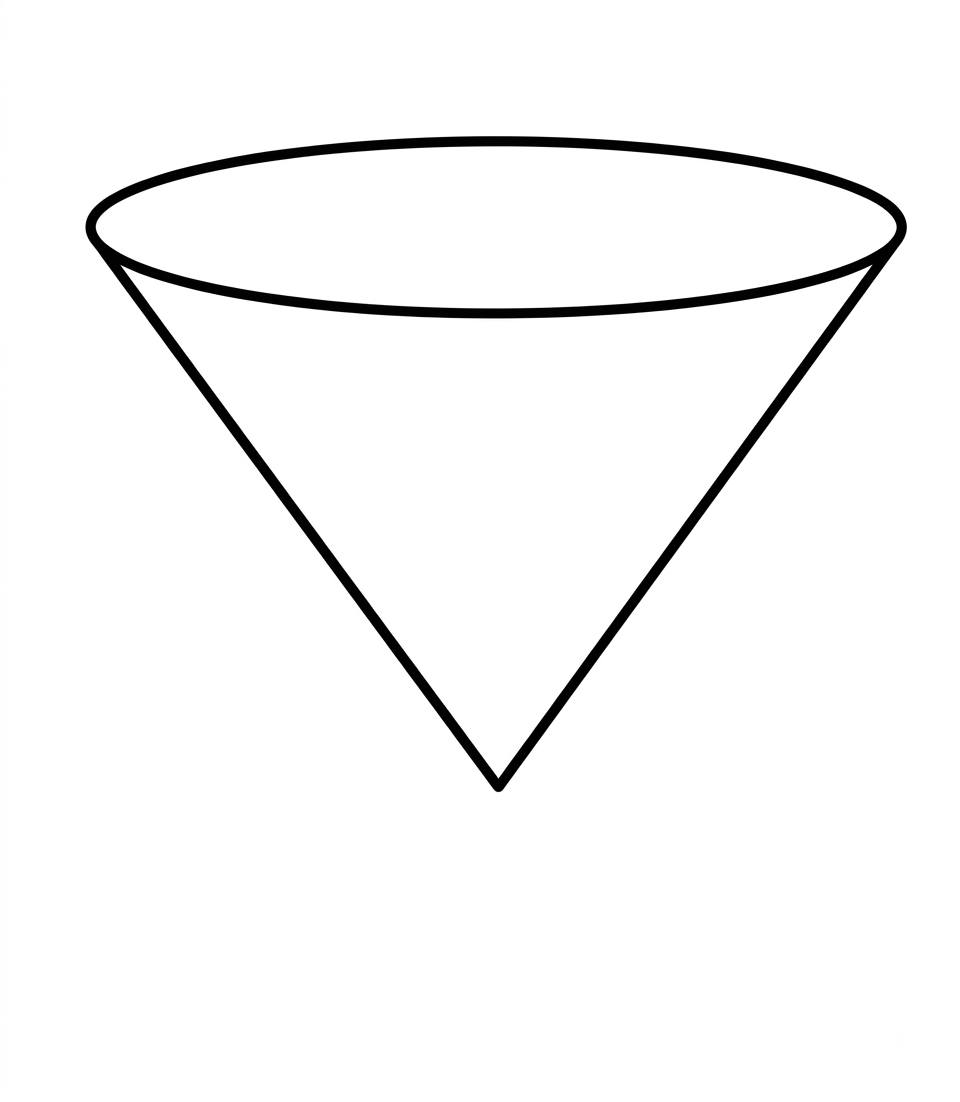
\includegraphics[width=0.3\textwidth]{../images/Hinhnon.png}
    
\end{figure}}
\newpage
\drawdashlines{33}
\newpage


% --- CÂU 5 ---
\questionShortAnswer{22}{2}{Thầy H có một cái bể hình chóp cụt đều với đáy dưới lớn hơn là hình vuông cạnh bằng 60 cm, đáy trên có cạnh bằng 30 cm và chiều cao bằng 100 cm. Ban đầu bể không có nước. Thầy H tiến hành bơm nước vào bể với tốc độ không đổi \( 2000 \, \text{cm}^3/\text{phút} \).  
 Hỏi tại thời điểm 10 phút, tốc độ dâng lên của mực nước trong bể bằng bao nhiêu? (đơn vị: cm/phút)(làm tròn đến hàng phần trăm)
 \begin{figure}[htbp]
    
    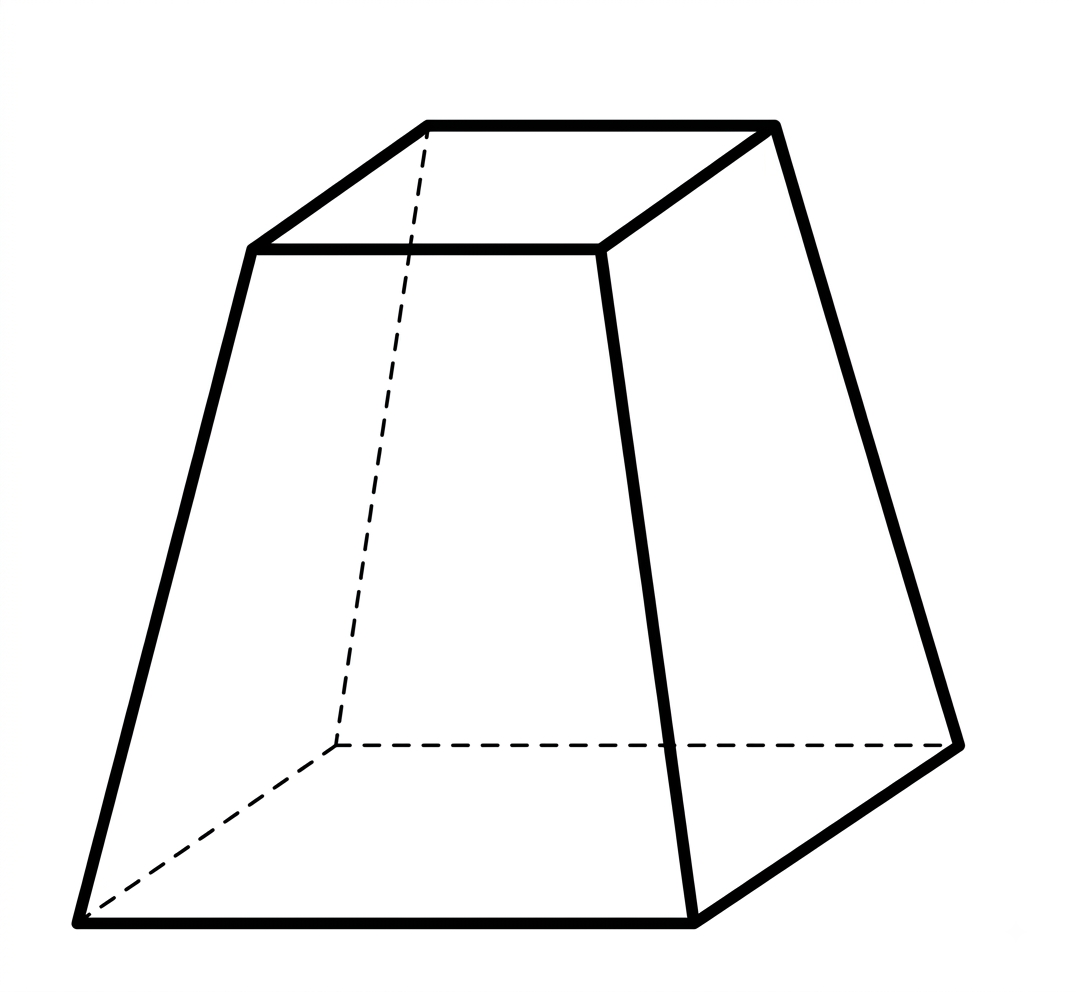
\includegraphics[width=0.3\textwidth]{../images/Chopcut.png}
    
\end{figure}}
\newpage
\drawdashlines{33}
\newpage


\end{document}